\subsection{Presentation des logiciels de test}

\subsubsection{Reconnaissance de formes simples dans un dessin}

Le premier logiciel que nous avons développé est un logiciel de reconnaissance de pictogrammes simples dans un dessin. L'affichage de ce logiciel est composé de deux parties : à gauche, le logiciel lit et affiche la vidéo. La partie droite de l'affichage sera utilisé pour afficher les captures de la vidéo sur lesquelles la détection a été faite.\\

À tout moment pendant la vidéo, un utilisateur peut prendre une capture d'image, à l'aide du bouton associé dans le logiciel. Lorsqu'une capture est prise, notre logiciel effectue des pré-traitements sur l'image obtenue, pour en améliorer la qualité, puis pour binariser l'image, et lance enfin l'analyse de template matching. Une fois l'analyse terminée, l'image obtenue est ajoutée à la liste des captures prises, que l'on peut voir entre les deux zones d'affichage. En cliquant sur le nom de cette capture, elle s'affiche dans la zone d'affichage de droite. Le résultat de l'analyse correspond à la capture prise dans la vidéo enrichie de boites englobantes autour des objets détectés.\\

Lorsque l'utilisateur a pris plusieurs captures, il est possible de naviguer entre ces différentes captures à l'aide des boutons situés entre les deux zones d'affichage.\\

Pour faciliter la prise de captures, nous permettons à l'utilisateur de mettre en pause la vidéo à l'aide de la touche espace.\\

\begin{center}
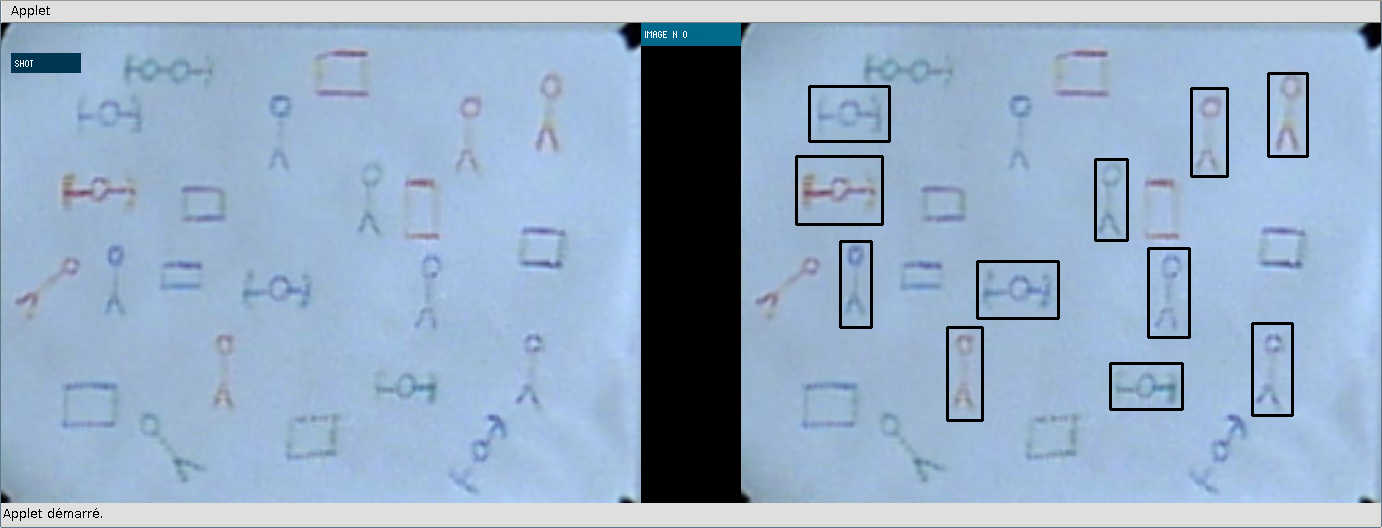
\includegraphics[width=\textwidth]{images/capture1.png}
\captionof{figure}{Présentation du logiciel de reconnaissance}
\end{center}

\subsubsection{Détection des évolutions d'un dessin}

Le second logiciel que nous avons développé est un logiciel de détection des évolutions dans le temps d'un dessin. L'affichage de ce logiciel est composé de trois zones d'affichage : les deux zones supérieures présentent les deux images qui sont comparées, ces zones sont séparées par la liste des images affichables. La zone inférieure présente le résultat de la différence entre les deux images.\\

Ce logiciel prend en entrée un dossier contenant différentes captures d'un dessin prises au cours du temps. À l'aide des boutons centraux, l'utilisateur peut choisir les deux images qu'il veut comparer. Une fois les deux images choisies, on peut lancer la comparaison à l'aide du bouton run. Une fois la comparaison achevée, le résultat s'affiche dans la zone inférieure. Ce résultat correspond à la différence entre les deux images d'origine binarisées. Le résultat est également stocké, afin d'éviter de recalculer l'image si l'utilisateur demande un calcul déjà fait.\\

\begin{center}
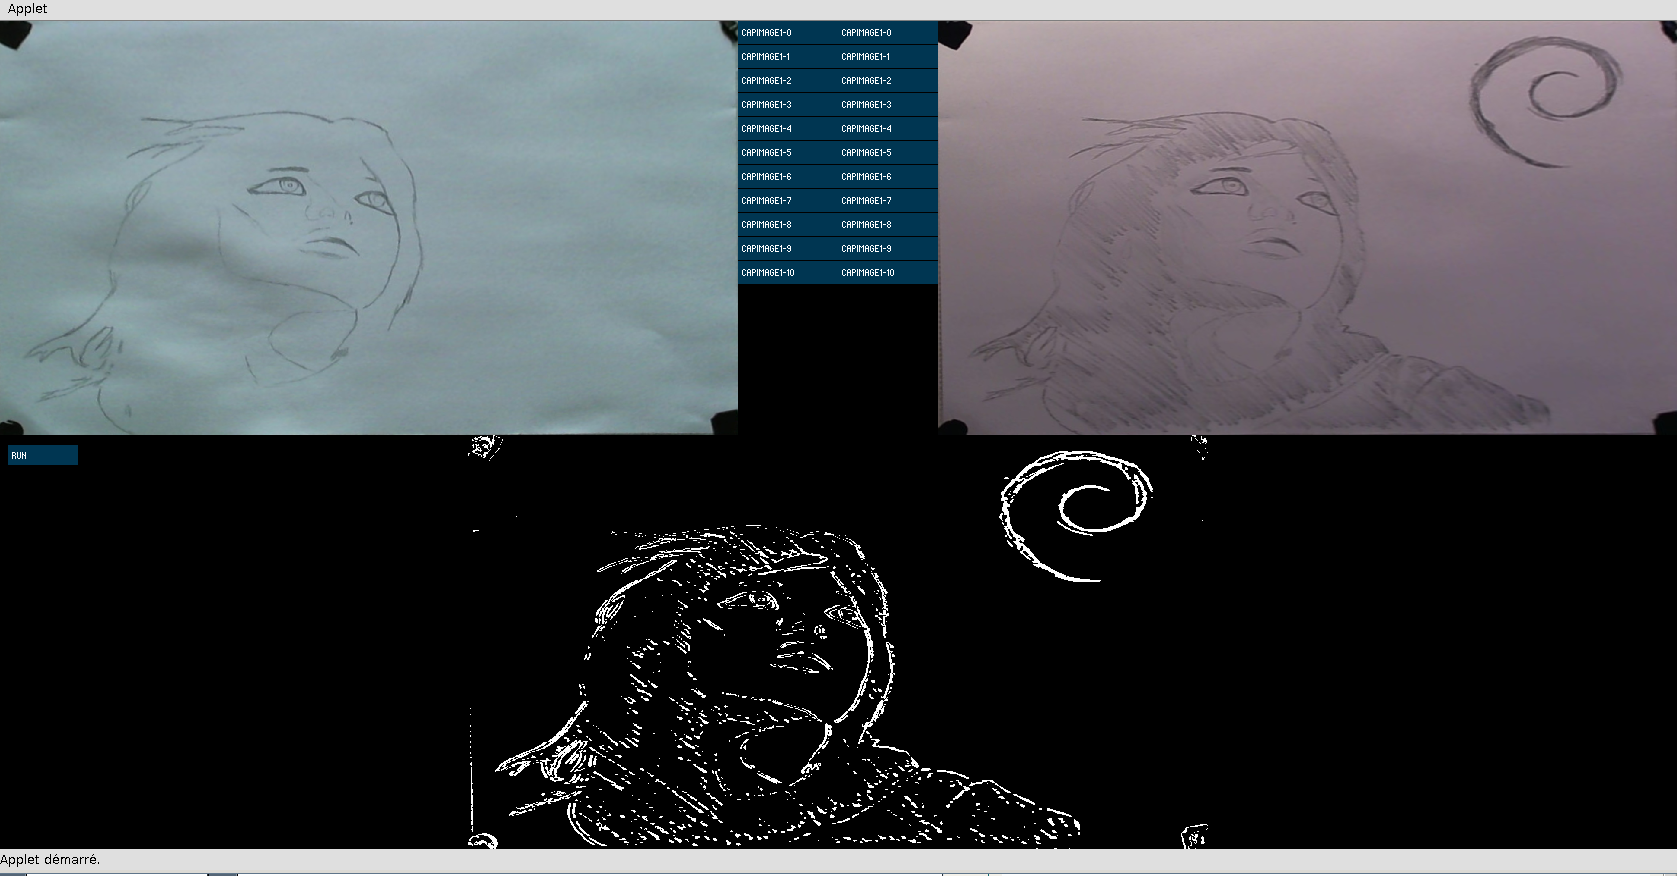
\includegraphics[width=\textwidth]{images/evolution1.png}
\captionof{figure}{Présentation du logiciel de détection d'évolutions}
\end{center}

\subsection{Résultats obtenus}